\chapter{Directed homologies}
\label{chap:dirhom}

The problem with homotopy groups is that they are hardly computable. Even given a finite presentation of a space, typically using pre-cubical or pre-simplicial sets, there is no nice way to compute their homotopy groups. For example, we would expect that the $n$th homotopy group to only depend on cells of small dimensions, typically lower than $n$ or $n+1$. But it is not the case: the $2$-sphere
$$S^2 =\{(t_0,t_1,t_2) \in \mathbb{R}^3 \mid 0 \leq t_i \leq 1 \wedge \sum t_i^2 = 1\}$$
can be presented (for example in pre-simplicial sets) using only cells of dimension lower than $2$. It can be proved that $S^2$ has infinitely many non-trivial homotopy groups. Consequently, homotopy groups do not depend on the ``cellular structure'' of a space.

Following an idea derived from the Euler characteristic, homology avoids this problem: homology can be defined directly on the cellular structure, for example, directly on a finite presentation, and was made to count things, typically, holes of a space. Let us illustrate this on a example from \cite{hatcher02}. Start with the following graph:
	\begin{figure}[H]
		\begin{center}
    			  \begin{tikzpicture}[auto,scale = 1.2]
%    \draw [fill = gray!25, draw = gray!75] (0,0) rectangle (1.4,1.4);
%    \node (c) at (0.7,0.7) {$A$};
%    \node   (x1) at (-0.2,-0.2) {\footnotesize{$s$}};
%    \node  (x2) at (1.6,-0.2) {\footnotesize{$s'$}};
%    \node  (x3) at (-0.2,1.6) {\footnotesize{$t$}};
%    \node  (x4) at (1.6,1.6) {\footnotesize{$t'$}};
%    \draw [thick] (0,0) to node [swap] {\footnotesize{$a$}} (1.4,0);
%    \draw [thick] (0,0) to node {\footnotesize{$b$}} (0,1.4);
%    \draw [thick] (1.4,0) to node [swap] {\footnotesize{$c$}} (1.4,1.4);
%    \draw [thick] (0,1.4) to node {\footnotesize{$d$}} (1.4,1.4);

	\draw (0,0) -- (0,2);
	\draw (-1,1)  to [bend right = 45] (0,0);
	\draw  (0,2) to [bend right = 45] (-1,1);
	\draw (0,0) to [bend right = 45] (1,1);
	\draw (0,2) to [bend left = 45] (1,1);
	\node at (0,0) {$\bullet$};
	\node at (0,2) {$\bullet$};
	\node[rotate=-90] at (0,1) {$\blacktriangleleft$};
	\node[rotate=-90] at (-1,1) {$\blacktriangleleft$};
	\node[rotate=-90] at (1,1) {$\blacktriangleleft$};
	\node at (0,-0.3) {\scriptsize{$0$}};
	\node at (0,2.3) {\scriptsize{$1$}};
	\node at (-1.2,1) {\scriptsize{$a$}};
	\node at (0.2,1) {\scriptsize{$b$}};
	\node at (1.2,1) {\scriptsize{$c$}};
  \end{tikzpicture}
  		\end{center}
	\end{figure}
\noindent Its geometric realization is three copies $a$, $b$, $c$ of the segment $[0,1]$ whose $0$ points (resp. $1$ points) are identified. Its fundamental group on $0$ is computed as follow. The path that follow $a$ forwardly and $b$ backwardly is not homotopic to the constant path. It is a generator of the fundamental group and let us note it $ab^{-1}$. Another generator is given by $cb^{-1}$ and those two are the only generators and there is no relation between them. Consequently, the fundamental group is the free group with two generators. Those generators represent the smallest cycles that cannot be squeezed to a point. If now we had a $2$-dimensional cell as follow:
	\begin{figure}[H]
		\begin{center}
    			\input{images/DirHom/HomEx2}
  		\end{center}
	\end{figure}
\noindent then the generator $ab^{-1}$ is killed since the path is now homotopic to the constant path and the fundamental group is then isomorphic to $\mathbb{Z}$. In those examples, the higher homotopy groups are all trivial. Assume now that we add another $2$-dimensional cell $B$ as follow:
	\begin{figure}[H]
		\begin{center}
    			  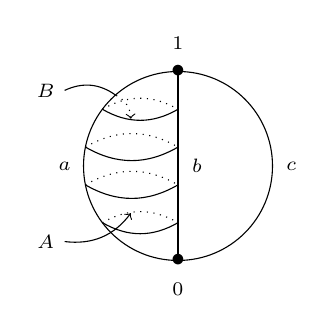
\begin{tikzpicture}[auto,scale = 1.2]
%    \draw [fill = gray!25, draw = gray!75] (0,0) rectangle (1.4,1.4);
%    \node (c) at (0.7,0.7) {$A$};
%    \node   (x1) at (-0.2,-0.2) {\footnotesize{$s$}};
%    \node  (x2) at (1.6,-0.2) {\footnotesize{$s'$}};
%    \node  (x3) at (-0.2,1.6) {\footnotesize{$t$}};
%    \node  (x4) at (1.6,1.6) {\footnotesize{$t'$}};
%    \draw [thick] (0,0) to node [swap] {\footnotesize{$a$}} (1.4,0);
%    \draw [thick] (0,0) to node {\footnotesize{$b$}} (0,1.4);
%    \draw [thick] (1.4,0) to node [swap] {\footnotesize{$c$}} (1.4,1.4);
%    \draw [thick] (0,1.4) to node {\footnotesize{$d$}} (1.4,1.4);

	\draw (0,0) -- (0,2);
	\draw (-1,1)  to [bend right = 45] (0,0);
	\draw  (0,2) to [bend right = 45] (-1,1);
	\draw (0,0) to [bend right = 45] (1,1);
	\draw (0,2) to [bend left = 45] (1,1);
	\node at (0,0) {$\bullet$};
	\node at (0,2) {$\bullet$};
	\node[rotate=-90] at (0,1) {$\blacktriangleleft$};
	\node[rotate=-90] at (-1,1) {$\blacktriangleleft$};
	\node[rotate=-90] at (1,1) {$\blacktriangleleft$};
	\node at (0,-0.3) {\scriptsize{$0$}};
	\node at (0,2.3) {\scriptsize{$1$}};
	\node at (-1.2,1) {\scriptsize{$a$}};
	\node at (0.2,1) {\scriptsize{$b$}};
	\node at (1.2,1) {\scriptsize{$c$}};
	\draw (-0.8,0.4) to [bend right = 30] (0,0.4);
	\draw (-0.98,0.8) to [bend right = 30] (0,0.8);
	\draw (-0.8,1.6) to [bend right = 30] (0,1.6);
	\draw (-0.98,1.2) to [bend right = 30] (0,1.2);
	\draw[dotted] (-0.8,0.4) to [bend left = 30] (0,0.4);
	\draw[dotted] (-0.98,0.8) to [bend left = 30] (0,0.8);
	\draw[dotted] (-0.8,1.6) to [bend left = 30] (0,1.6);
	\draw[dotted] (-0.98,1.2) to [bend left = 30] (0,1.2);
	\draw[->] (-1.2,0.2) to [bend right = 30] (-0.5,0.5);
	\node at (-1.4,0.2) {\scriptsize{$A$}};
	\node at (-1.4,1.8) {\scriptsize{$B$}};
	\draw[dotted,<-] (-0.5,1.5) to [bend right = 30] (-0.66,1.75);
	\draw (-1.2,1.8) to [bend left = 30] (-0.66,1.75);
  \end{tikzpicture}
  		\end{center}
	\end{figure}
The fundamental group is still $\mathbb{Z}$ but now, higher generators are created: there is a continuous function from $\Box_2$ which ``covers'' $A$ and $B$ and which cannot be deformed to a constant function. This gives a generator of $\pi_2$. As said previously on the $2$-sphere, this also creates generators for infinitely many other homotopy groups.

Now imagine that we want to compute holes directly on the cellular structure. We will do this using abelian groups. Start with the first graph. With abelian notation, the generators are $a-b$ and $c-b$. Actually, the elements generated by those two are the combinations $n.a+m.b+p.c$ with $n$, $m$, $p$ integers and $n+p+m = 0$. Equivalently, if $\mathbb{Z}[a,b,c]$ (resp. $\mathbb{Z}[0,1]$) denotes the free abelian group generated by $a$, $b$ and $c$ (resp. $0$ and $1$) and $\partial_1$ denotes the morphism from $\mathbb{Z}[a,b,c]$ to $\mathbb{Z}[0,1]$ which maps $a$, $b$ and $c$ to $1 - 0$, then those elements are precisely the kernel of $\partial_1$. $\partial_1$ is a boundary map and the generated elements are those without boundary. Let us call them cycles. Now add the $2$-cell $A$ as previously. We are interested in holes, that we may think as cycles that cannot be filled. This can also be expressed as boundary maps: the boundary of the cell $A$ is precisely $a-b$ (modulo orientation). This means that the generator $a-b$ can be filled with the cell $A$. More precisely, there is a map $\partial_2$ from $Z[A]$ to $Z[a,b,c]$ which maps $A$ to $a-b$. The cycles that can be filled are precisely the image of $\partial_2$. Actually, notice that $\text{Im} \partial_2 \subseteq \text{Ker} \partial_1$. We can then form the group $\text{Ker} \partial_1 / \text{Im} \partial_2$ which will have one generator $c-b$, which stands for a $1$-dimensional hole. This will be the definition of the first homology group. Similarly, if we add the second $2$-cell $B$, $\partial_2$ will be from $\mathbb{Z}[A,B]$ and will map $B$ to $a-b$. $\text{Ker} \partial_1 / \text{Im} \partial_2$ still have one generator but now $\partial_2$ has a non-trivial kernel ($A-B$ is a generator) which creates a generator for a second homology group, which stands for a $2$-dimensional hole. And if we add higher dimensional cells we can continue this process to define a sequence of groups as quotients $\text{Ker} \partial_n/\text{Im} \partial_{n+1}$ of boundary maps.

In this chapter, we will recall the definition of singular homology of a topological space (Section \ref{subsec:homdef}) and see some of its properties: it is an invariant of homotopy (Section \ref{subsec:hominv}), it is complete in some cases (Section \ref{subsec:hurwhi}), it is modular (Section \ref{subsec:eilste}) and it is computable (Section \ref{subsec:homcom}). We would then define a similar theory for directed spaces. We start, in Section \ref{sec:exidirhom}, by presenting a few candidates proposed in the literature and explain why we are not happy with them. We then describe our own candidates: starting with the idea that what matter are the dipath/trace spaces and how they evolve with time (Section \ref{sec:traspaevo}), we construct several diagrams, namely functors from any small category to a specified category (typically, a category of modules), which represent the homology of the trace spaces of a d-space and how they evolve when extending traces, called natural and bimodule homologies (Section \ref{sec:nathom}). Finally, in Section \ref{sec:homdiag}, we look at first nice properties of this homology theory: first invariance under dihomotopy and several Eilenberg-Steenrod axioms, in particular, we will see what can be said about modularity using the theory of exactness in non-Abelian theories from \cite{grandis91}.

\section{Classical homology and a few properties}


The goal of this section is to briefly present the theory of homology in classical algebraic topology. For a general study, see for example \cite{hatcher02}. 

\subsection{Definitions}
\label{subsec:homdef}

Homology is a general technique to measure default of exactness in a sequence of morphisms. We start here by looking at the case of $\R$-modules for a certain ring $\R$ (we will see a more general framework soon). We note $\modu{\R}$ the categories of $\R$-modules and linear maps. The notion of exact sequence is important in algebra since many properties can be expressed using it. Precisely:


\begin{defi}
Let $\map{f}{A}{B}$ and $\map{g}{B}{C}$ be linear maps. We say that the following sequence:
\begin{center}
\begin{tikzpicture}
  \matrix (m) [matrix of math nodes,row sep=4em,column sep=4em,minimum width=2em]
  {
     
A &
B &
C
    \\};
  \path[-stealth]
    (m-1-1) edge node [above] {$f$} (m-1-2)
    (m-1-2) edge node [above] {$g$} (m-1-3);
\end{tikzpicture}
\end{center}
is \textbf{exact} if $Im(f) = Ker(g)$.
We say that it is \textbf{short exact} if, furthermore, $f$ is injective and $g$ is surjective.
We say that the following sequence 
\begin{center}
\begin{tikzpicture}
  \matrix (m) [matrix of math nodes,row sep=4em,column sep=4em,minimum width=2em]
  {
   
\cdots &
A_n &  
\cdots &
A_1 &
A_0
    \\};
  \path[-stealth]
    (m-1-1) edge node [above] {$f_{n+1}$} (m-1-2)
    (m-1-2) edge node [above] {$f_n$} (m-1-3)
    (m-1-3) edge node [above] {$f_2$} (m-1-4)
    (m-1-4) edge node [above] {$f_1$} (m-1-5);
\end{tikzpicture}
\end{center}
is \textbf{long exact} if for every $n\in \mathbb{N}$, the sequence:
\begin{center}
\begin{tikzpicture}
  \matrix (m) [matrix of math nodes,row sep=4em,column sep=4em,minimum width=2em]
  {
     
A_{n+2} &
A_{n+1} &
A_n
    \\};
  \path[-stealth]
    (m-1-1) edge node [above] {$f_{n+2}$} (m-1-2)
    (m-1-2) edge node [above] {$f_{n+1}$} (m-1-3);
\end{tikzpicture}
\end{center}
is exact.
\end{defi}
 
As announced, we want to look at default of exactness of sequences of linear maps. We call \textbf{chain complex} a sequence $C = (\map{\partial_{n+1}}{C_{n+1}}{C_n})_{n\in\mathbb{N}}$ of linear maps such that for every $n \in \nat$, $\partial_n\circ\partial_{n+1} = 0$. In particular, this implies that $Im(\partial_{n+1}) \subseteq Ker(\partial_n)$. So a chain complex is exact precisely when all the quotients $Ker(\partial_n)/Im(\partial_{n+1})$ are trivial. We then use those quotients to measure the default of exactness: we call \textbf{$n$th module of homology} and denote by $H_n(C)$ the quotient $Ker(\partial_n)/Im(\partial_{n+1})$ (by convention $H_0(C) = C_0/Im(\partial_1)$).

A morphism of chain complexes
$$\map{(f_n)_{n\in\mathbb{N}}}{(\map{\partial_{n+1}}{C_{n+1}}{C_n})_{n\in\mathbb{N}}}{(\map{\partial'_{n+1}}{C'_{n+1}}{C'_n})_{n\in\mathbb{N}}}$$
is a sequence of linear maps $(\map{f_n}{C_n}{C'_n})_{n\in\mathbb{N}}$ such that for every $n \in \nat$, 
$$f_n \circ \partial_{n+1} = \partial'_{n+1} \circ f_{n+1}.$$
We denote by $\chain{\modu{\R}}$ the category of chain complexes of $\R$-modules and morphisms of chain complexes.

$H_n$ extends to a functor from $\chain{\modu{\R}}$ to $\modu{\R}$ by defining $\map{H_n((f_k)_{k\in\mathbb{N}})}{H_n(C)}{H_n(C')}$ as the linear map $[x] \mapsto [f_n(x)]$ (where $[x]$ is the class of $x\in Ker ~ \partial_{n-1}$ in $H_n(C)$).
 
In algebraic topology, we study the geometry of a space using a particular chain complex, called the \textbf{singular chain complex}. Recall the $\sing$ functor from Section \ref{subsec:hohy}. It is a functor from $\topo$ to $\sset$ which maps a topological space $X$ to a simplicial set such that $\sing(X)_n$ is the set of continuous functions from $\Delta_n$ to $X$. Recall also the face maps $\map{d_i}{\sing(X)_{n+1}}{\sing(X)_n}$ are defined as $d_i(\alpha) = \alpha\circ\partial_i$, where $\map{\partial_i}{\Delta_n}{\Delta_{n+1}}$ is the corresponding geometric face map, that is the inclusion of the $i$-th face into the $n$-th standard geometric simplex. The singular chain complex $C(X)$ is then defined as follow:
\begin{itemize}
	\item for $n\in\nat$, $C_n(X)$ is the free module generated by $\sing(X)_n$,
	\item $\map{\partial_{n+1}}{C_{n+1}(X)}{C_n(X)}$ is the linear map such that for every $\alpha \in C_{n+1}(X)$, $$\partial(\alpha) = \sum\limits_{i=0}^{n+1} (-1)^i d_i(\alpha).$$
\end{itemize}
The \textbf{$n$th module of singular homology of $X$}, denoted by $H_n(X)$, is defined as $H_n(C(X))$. $C$ and $H_n$ extends to functors from $\topo$ to respectively $\chain{\modu{\R}}$ and $\modu{\R}$.

Intuitively, the homology of a space computes the number of holes of any dimension of this space. For example, a space has a hole of dimension $1$, if the image of the boundary of a triangle by a continuous function cannot be extended in a continuous function from the whole triangle. For example, $\mathbb{R}^2\setminus\{0\}$ has a hole of dimension $2$. Similarly, $n$-spheres have a hole of dimension $n$. From the homology point of view, this means that their $n$th homology module is isomorphic to $\R$.

Given a pair $(X,A)$ in $\topp$, there is an injection from $C(A)$ into $C(X)$ and one can form the quotient $C(X)/C(A)$ which defines a chain complex called the \textbf{chain complex of $X$ relative to $A$}. We note $H_n(X,A) = H_n(C(X)/C(A))$ and called it the \textbf{$n$th module of homology of $X$ relative to $A$}. Intuitively, it computes the algebraic informations of $X$ modulo $A$ and is useful to know more precisely where the various bits of information on $X$ are located. $H_n$ extends to a functor from $\topp$ to $\modu{\R}$. Remark that in particular, $H_n(X) = H_n(X,\varnothing)$.

For every $i \geq 1$, there is a natural linear map $\map{\delta_i}{H_i(X,A)}{H_{i-1}(A)}$ defined as follow. The kernel of $\map{\partial_i}{C_i(X)/C_i(A)}{C_{i-1}(X)/C_{i-1}(A)}$ is precisely the class of elements $\alpha$ of $C_i(X)$ such that $\partial_i(\alpha)$ is included in $A$. Since $C(A)$ is a chain complex, $\partial_i(\alpha)$ belongs to $Ker \partial_{i-1}$. This process behaves well modulo $\Ima \partial_i$ and so defines a linear map from $H_i(X,A)$ to $H_{i-1}(A)$.


\subsection{Homotopy invariance}
\label{subsec:hominv}

The theorem of homotopy invariance of the homology is a correction result:

\begin{theo}[\cite{hatcher02}] If two continuous maps from $X$ to $Y$ are homotopic then the linear maps induced on homology coincide. In particular, if $X$ and $Y$ are homotopically equivalent then homology are isomorphic.\end{theo}

\subsection{Hurewicz and Whitehead theorems}
\label{subsec:hurwhi}

Reciprocally, in the case $\R = \ZZ$, the homology is not that far from homotopy:

\begin{theo}[Hurewicz \cite{hatcher02}] Let $X$ be a topological space. Then:
\begin{itemize}
	\item $H_0(X)$ is isomorphic to the free Abelian group generated by $\pi_0(X)$, that is, to $\bigoplus\limits_{\pi_0(X)}\mathbb{Z}$,
	\item if $X$ is $(n-1)$-connected, i.e., for every $1\leq i \leq n-1$ and every $x\in X$, $\pi_i(X,x)$ is trivial and $\pi_0(X)$ is a singleton then: 
		\begin{itemize}
			\item if $n=1$, $H_1(X)$ is isomorphic to the abelianization of $\pi_1(X)$,
			\item otherwise, $H_n(X)$ and $\pi_n(X)$ are isomorphic.
		\end{itemize}
\end{itemize}
Moreover, those isomorphisms are natural in $X$.
\end{theo}

\begin{theo}[Whitehead \cite{spanier66}] Let $X$ and $Y$ be two simply-connected (i.e., $1$-connected) CW-complexes. If a continuous function $\map{f}{X}{Y}$ induces an isomorphism in homology, i.e., for every $n\in \mathbb{N}$, $\map{H_n(f)}{H_n(X)}{H_n(Y)}$ is an isomorphism, then $X$ and $Y$ are homotopically equivalent.
\end{theo}

\subsection{Eilenberg-Steenrod axioms}
\label{subsec:eilste}

Eilenberg and Steenrod isolated in \cite{eilenberg45} a few common properties of the different homology theories that can be defined on topological spaces and which are enough to prove main results about those theories. Those properties were stated for theories with values in Abelian groups (or $\ZZ$-modules), but can actually be stated more generally in Abelian categories ($\modu{\R}$ is such a category) or even in more general frameworks as we will see later. We will stick here to categories of modules. 

A \textbf{homology theory} is a family $(H_n)_{n\in \nat}$ of functors from $\topp$ to $\modu{\R}$, together with a family of natural transformations $\partial_n$ from $H_n$ to the functor $(X,A) \mapsto H_{n-1}(A,\varnothing)$. We say that a homology theory satisfies the \textbf{Eilenberg-Steenrod axioms} if it satisfies the following:
\begin{itemize}
	\item \textbf{homotopy axiom:} if two maps $\map{f,g}{(X,A)}{(Y,B)}$ are homotopic then $H_n(f) = H_n(g)$ for every $n$. In particular, homotopy equivalences induce isomorphisms between homology modules.
	\item \textbf{excision axiom:} for every pair $(X,A)$ and every open subset $U$ of $X$ such that the closure of $U$ is included in the interior of $A$ and if $\iota$ denotes the inclusion from $(X\setminus U,A\setminus U)$ to $(X,A)$ then $H_n(\iota)$ is an isomorphism for every $n$,
	\item \textbf{dimension axiom:} $H_n(\ast,\varnothing)$ is a trivial module for every $n \neq 0$,
	\item \textbf{additivity axiom:} for every $n$, the functor $\map{H_n}{\topo}{\modu{\R}}$ which maps $X$ to $H_n(X,\varnothing)$ preserves coproducts,
	\item \textbf{exactness axiom:} for every pair $(X,A)$, the following sequence:
	\begin{figure}[H]
		\begin{center}
    			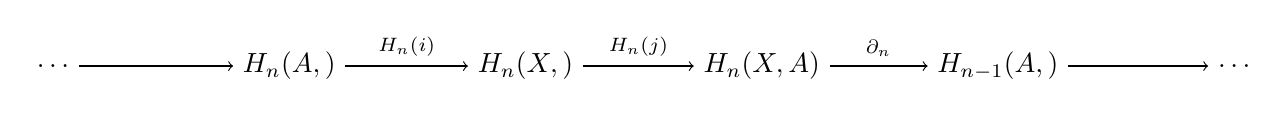
\begin{tikzpicture}

	\node (0) at (0,0) {$\ldots$};
	\node (1) at (3,0) {$H_n(A,\varnothing)$};
	\node (2) at (6,0) {$H_n(X,\varnothing)$};
	\node (3) at (9,0) {$H_n(X,A)$};
	\node (4) at (12,0) {$H_{n-1}(A,\varnothing)$};
	\node (5) at (15,0) {$\ldots$};
	
	\path[->, font=\scriptsize]
		(0) edge (1)
		(1) edge node[above]{$H_n(i)$} (2)
		(2) edge node[above]{$H_n(j)$} (3)
		(3) edge node[above]{$\partial_n$} (4)
		(4) edge (5);

\end{tikzpicture}
  		\end{center}
	\end{figure}
	\vskip -0.5cm
	is long exact, where $i$ is the inclusion from $(A,\varnothing)$ to $(X,\varnothing)$ and $j$ is the inclusion from $(X,\varnothing)$ to $(X,A)$.
\end{itemize}

Singular homology is a homology theory that satisfies the Eilenberg-Steenrod axioms. Actually, the exactness axiom can be extended in the following way. Let us say that a sequence of morphisms of chain complexes of the form:
\begin{center}
\begin{tikzpicture}
  \matrix (m) [matrix of math nodes,row sep=4em,column sep=4em,minimum width=2em]
  {
     
A &
B &
C
    \\};
  \path[-stealth]
    (m-1-1) edge node [above] {$(f_n)_{n\in\mathbb{N}}$} (m-1-2)
    (m-1-2) edge node [above] {$(g_n)_{n\in\mathbb{N}}$} (m-1-3);
\end{tikzpicture}
\end{center}
is \textbf{(short) exact} if for every $n$, the sequence:
\begin{center}
\begin{tikzpicture}
  \matrix (m) [matrix of math nodes,row sep=4em,column sep=4em,minimum width=2em]
  {
     
A_n &
B_n &
C_n
    \\};
  \path[-stealth]
    (m-1-1) edge node [above] {$f_n$} (m-1-2)
    (m-1-2) edge node [above] {$g_n$} (m-1-3);
\end{tikzpicture}
\end{center}
is (short) exact. One can observe that the sequence:
\begin{center}
\begin{tikzpicture}
  \matrix (m) [matrix of math nodes,row sep=4em,column sep=4em,minimum width=2em]
  {
     
C(A) &
C(X) &
C(X)/C(A)
    \\};
  \path[-stealth]
    (m-1-1) edge node [above] {$i$} (m-1-2)
    (m-1-2) edge node [above] {$q$} (m-1-3);
\end{tikzpicture}
\end{center}
where $i$ is the injection and $q$ the quotient map, is short exact. The fact that this particular short exact sequence of chain complexes induces a long exact sequence of homology is more general:

\begin{theo}[\cite{hatcher02}]
If \begin{center}
\begin{tikzpicture}
  \matrix (m) [matrix of math nodes,row sep=4em,column sep=4em,minimum width=2em]
  {
     
A &
B &
C
    \\};
  \path[-stealth]
    (m-1-1) edge node [above] {$f$} (m-1-2)
    (m-1-2) edge node [above] {$g$} (m-1-3);
\end{tikzpicture}
\end{center}
is a short exact sequence of chain complexes then there is a long exact sequence of the form:
\begin{center}
\begin{tikzpicture}
  \matrix (m) [matrix of math nodes,row sep=4em,column sep=3.5em,minimum width=2em]
  {
     \ldots & 
H_{n}(B) &
H_{n}(C) &
H_{n-1}(A) &
H_{n-1}(B) &
\ldots
    \\};
  \path[-stealth]
    (m-1-1) edge node [above] {} (m-1-2)
    (m-1-2) edge node [above] {$H_n(g)$} (m-1-3)
    (m-1-3) edge node [above] {} (m-1-4)
    (m-1-4) edge node [above] {$H_{n-1}(f)$} (m-1-5)
    (m-1-5) edge node [above] {} (m-1-6);
\end{tikzpicture}
\end{center}
\end{theo}

One of the important theorem that can be proved from the Eilenberg-Steenrod axioms is the following:

\begin{theo}[Mayer-Vietoris \cite{hatcher02}] Let $A,B \subseteq X$ be spaces such that the union of the interiors of $A$ and $B$ covers $X$ Then, there is a long exact sequence of the form: 

\begin{center}
\begin{tikzpicture}
  \matrix (m) [matrix of math nodes,row sep=4em,column sep=3em,minimum width=2em]
  {
     \ldots & 
H_{n}(A\cap B) &
H_{n}(A) \bigoplus H_{n}{B} &
H_{n}(X) &
H_{n-1}(A\cap B) &
\ldots
    \\};
  \path[-stealth]
    (m-1-1) edge node [above] {} (m-1-2)
    (m-1-2) edge node [above] {} (m-1-3)
    (m-1-3) edge node [above] {} (m-1-4)
    (m-1-4) edge node [above] {} (m-1-5)
    (m-1-5) edge node [above] {} (m-1-6);
\end{tikzpicture}
\end{center}
\end{theo}



\subsection{Computability}
\label{subsec:homcom}

The main interest of homology is that it is computable when the space is finitely presented, typically by a finite presimplicial set. The main ingredient is that, when $\R$ is a principal ideal domain, the finitely generated modules are isomorphic to a module of the form $\R/(\alpha_1)\times ... \times\R/(\alpha_k)$ where $(\alpha)$ is the ideal generated by $\alpha$ and with $(\alpha_1) \subseteq \ldots \subseteq (\alpha_k)$, and this form is unique. So when the space is presented by a finite presimplicial set, its homology is isomorphic to a finitely generated module computed from the presimplicial structure, and from this structure it is possible to compute those $\alpha_1$ when $\R \in \{\RR,\QQ,\ZZ\}$. When $\R \in \{\RR,\QQ\}$ those module are in fact vector spaces of finite dimension and so isomorphic to $\RR^p$ (resp. $\QQ^p$) for some $p$. We call those integers the \textbf{Betti numbers}. When $\R = \ZZ$, it is isomorphic to an Abelian group of the form $\mathbb{Z}^\beta\times\mathbb{Z}/\alpha_1\mathbb{Z}\times ... \mathbb{Z}/\alpha_k\mathbb{Z}$ with $2 \leq \alpha_1|...|\alpha_k$. The $\alpha_i$ are called \textbf{torsion coefficients}. It is possible to compute those integers computing Smith normal form, see \cite{munkres30}. 

Another tool to compute homology is the Mayer-Vietoris theorem. This theorem means that homology is modular: in some cases, it is possible to express the homology of some spaces using simpler spaces. It is, for example, possible to compute homology of spheres using this theorem. Indeed, a $n$-sphere is the union of two contractible spaces (the 2 hemispheres) whose intersection is (up to homotopy equivalence) a $n-1$-sphere, and by the Mayer-Vietoris, it is possible to compute by induction those homology modules: $H_n(S^n) \simeq \ZZ$ and for $k \neq n$, $H_k(S^n) \simeq 0$.




\section{Existing directed homologies}
\label{sec:exidirhom}

Since \cite{goubault95}, different definition of directed homologies were proposed for various frameworks. From a theoretical point of view, we would like to construct a homology theory which satisfies as many good properties (for example, those presented earlier for classical homology) as possible. Among those, here are a few:
\begin{itemize}
	\item directed homology must be an invariant of directed homotopy. Here it does depend on the dihomotopy theory considered. In our case, it would be the inessential theory.
	\item directed homology should detect default of dihomotopy and not be too far from homotopy. Typically, we would like that spaces much as the matchbox (which is not inessentially equivalent to a point) not to have a trivial directed homology.
	\item directed homology should be modular or at least be with values in a category where the theory of exact sequences should be nice.
	\item directed homology should be, somehow, computable in some cases.
\end{itemize}

\noindent Among the proposition, we could mention:
\begin{itemize}
	\item the branching, confluent and total homologies from \cite{goubault95}. They were made for studying geometric properties of HDA. They are computable but they lack of directedness, since they are essentially invariant by undirected equivalence.
	\item the directed homology from \cite{grandis04}. It is constructed by equipping homology groups with an order. If you have in mind that the generators of those groups are holes, the order represents how those holes are located from one to the other. It is invariant by directed equivalence (it was made for this). For example, the matchbox has a trivial directed homology in this case since it is classically contractible, so its singular homology is trivial, and only trivial structures can be equipped on trivial groups.
	\item the directed homology \cite{fahrenberg03}, using $\omega$-categories. Fahrenberg observed that the homology of the matchbox was trivial.
	\item the homology graph from \cite{kahl14}. The idea is similar to \cite{grandis04}, except that groups are equipped with more general relations. Kahl proved that it is invariant by an analogue of homeomorphisms for pre-cubical sets. The matchbox has a trivial homology graph for the same reason as Grandis' proposal.
	\item the homology with values in cancellative monoids from \cite{patchkoria06}. Since cancellative monoids only catch cancellative behaviors, it is not satisfactory for our purpose.
	\item directed (co)homology from \cite{ghrist16}. It was made for a completely different purpose (solve pursuit-evasions problem) and does not seem to relate to our goal.
\end{itemize}





\section{Trace spaces and evolution}
\label{sec:traspaevo}

We have seen that trace spaces are good abstractions for a space of ``executions'' of a truly concurrent system. They give interesting information about the space. However, limiting ourself to only one trace space is not sufficient to classify spaces. Let us look at those two d-spaces, which are geometric realizations of $SU$-programs:
	\begin{figure}[H]
		\begin{center}
    			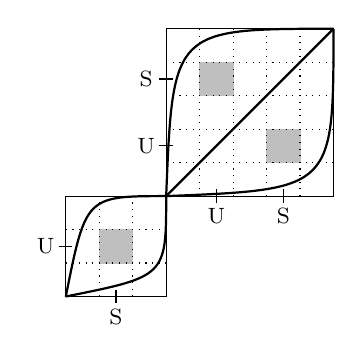
\begin{tikzpicture}[auto,scale = 0.85]
\draw (0,0) rectangle (1.5,1.5);
\draw (1.5,1.5) rectangle (4,4);
\draw [fill = gray!50,draw = gray!50] (0.5,0.5) rectangle (1,1);
\draw [fill = gray!50,draw = gray!50] (2,3) rectangle (2.5,3.5);
\draw [fill = gray!50,draw = gray!50] (3,2) rectangle (3.5,2.5);
\draw [dotted] (1,0) to (1,1.5);
\draw [dotted] (0.5,0) to (0.5,1.5);
\draw [dotted] (0,1) to (1.5,1);
\draw [dotted] (0,0.5) to (1.5,0.5);
\draw [dotted] (2,1.5) to (2,4);
\draw [dotted] (2.5,1.5) to (2.5,4);
\draw [dotted] (3,1.5) to (3,4);
\draw [dotted] (3.5,1.5) to (3.5,4);
\draw [dotted] (1.5,2) to (4,2);
\draw [dotted] (1.5,2.5) to (4,2.5);
\draw [dotted] (1.5,3) to (4,3);
\draw [dotted] (1.5,3.5) to (4,3.5);
\draw (0.75,-0.1) to (0.75,0.1);
\draw (-0.1,0.75) to (0.1,0.75);
\draw (2.25,1.4) to (2.25,1.6);
\draw (3.25,1.4) to (3.25,1.6);
\draw (1.4,2.25) to (1.6,2.25);
\draw (1.4,3.25) to (1.6,3.25);
\node (S11) at (0.75,-0.3) {\footnotesize{S}};
\node (U21) at (-0.3,0.75) {\footnotesize{U}};
\node (U11) at (2.25,1.2) {\footnotesize{U}};
\node (S12) at (3.25,1.2) {\footnotesize{S}};
\node (U22) at (1.2,2.25) {\footnotesize{U}};
\node (S21) at (1.2,3.25) {\footnotesize{S}};
\draw [thick] (0,0) .. controls (0.3,1.5)  .. (1.5,1.5);
\draw [thick] (0,0) .. controls (1.5,0.3)  .. (1.5,1.5);
\draw [thick] (1.5,1.5) to (4,4);
\draw [thick] (1.5,1.5) .. controls (1.6,4)  .. (4,4);
\draw [thick] (1.5,1.5) .. controls (4,1.6)  .. (4,4);
\end{tikzpicture}
\begin{tikzpicture}
\draw[color = white] (0,-1) rectangle (3,-1.1);
\end{tikzpicture}
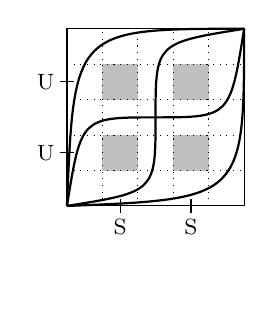
\begin{tikzpicture}[auto,scale = 0.9]
\draw (0,0) rectangle (2.5,2.5);
\draw [fill = gray!50,draw = gray!50] (0.5,0.5) rectangle (1,1);
\draw [fill = gray!50,draw = gray!50] (0.5,1.5) rectangle (1,2);
\draw [fill = gray!50,draw = gray!50] (1.5,0.5) rectangle (2,1);
\draw [fill = gray!50,draw = gray!50] (1.5,1.5) rectangle (2,2);
\draw [dotted] (1,0) to (1,2.5);
\draw [dotted] (0.5,0) to (0.5,2.5);
\draw [dotted] (1.5,0) to (1.5,2.5);
\draw [dotted] (2,0) to (2,2.5);
\draw [dotted] (0,1) to (2.5,1);
\draw [dotted] (0,0.5) to (2.5,0.5);
\draw [dotted] (0,1.5) to (2.5,1.5);
\draw [dotted] (0,2) to (2.5,2);
\draw (0.75,-0.1) to (0.75,0.1);
\draw (-0.1,0.75) to (0.1,0.75);
\draw (1.75,-0.1) to (1.75,0.1);
\draw (-0.1,1.75) to (0.1,1.75);
\node (S11) at (0.75,-0.3) {\footnotesize{S}};
\node (U21) at (-0.3,0.75) {\footnotesize{U}};
\node (S12) at (1.75,-0.3) {\footnotesize{S}};
\node (U22) at (-0.3,1.75) {\footnotesize{U}};
\draw [thick] (0,0) .. controls (0.2,1.25)  .. (1.25,1.25);
\draw [thick] (0,0) .. controls (1.25,0.2)  .. (1.25,1.25);
\draw [thick] (2.5,2.5) .. controls (1.25,2.3)  .. (1.25,1.25);
\draw [thick] (2.5,2.5) .. controls (2.3,1.25)  .. (1.25,1.25);
\draw [thick] (0,0) .. controls (0.1,2.5)  .. (2.5,2.5);
\draw [thick] (0,0) .. controls (2.5,0.1)  .. (2.5,2.5);
\node (b) at (0,-1) {};
\end{tikzpicture}
  		\end{center}
	\end{figure}
Both d-spaces have a trace space between their extremal points homotopically equivalent to a six point space. From a computer science point of view, this means that they have six maximal non-equivalent executions, depicted in both pictures. So if we were to only consider those trace spaces, we would not be able to distinguish those two spaces/programs, while they should be. From a computer science point of view, the observations from those two programs are different. From a mathematical point of view, those spaces are not even homotopically equivalent since they do not have the same number of holes.

\noindent In the following, much as \cite{raussen07}, we will study a structure which will allow us to look at all the trace spaces between two points and how their geometries evolve when varying their end points. More precisely, we will:
\begin{itemize}
	\item organize traces following the extension relation. This will be done by considering the category of factorizations or the enveloping category of the trace category from section \ref{subsec:trpacat},
	\item associate each trace or each pair of points (depending on which structure we use) with the trace space between its end points. This will define a functor from the structure from the first point to the category of topological spaces.
	\item apply homotopy group or homology module functors.
\end{itemize}

These ideas will be developed in the next section, but let us look at the previous example and show how these ideas will solve our problem. Being able to observe all the trace spaces between two points allow us to distinguish the two previous d-spaces. Indeed, if we look at the trace space between $\alpha$ and $\beta$ in the left example:
	\begin{figure}[H]
		\begin{center}
    			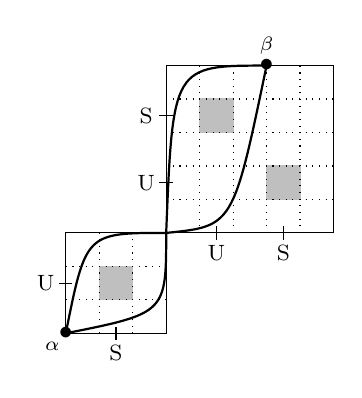
\begin{tikzpicture}[auto,scale = 0.85]
\draw (0,0) rectangle (1.5,1.5);
\draw (1.5,1.5) rectangle (4,4);
\draw [fill = gray!50,draw = gray!50] (0.5,0.5) rectangle (1,1);
\draw [fill = gray!50,draw = gray!50] (2,3) rectangle (2.5,3.5);
\draw [fill = gray!50,draw = gray!50] (3,2) rectangle (3.5,2.5);
\draw [dotted] (1,0) to (1,1.5);
\draw [dotted] (0.5,0) to (0.5,1.5);
\draw [dotted] (0,1) to (1.5,1);
\draw [dotted] (0,0.5) to (1.5,0.5);
\draw [dotted] (2,1.5) to (2,4);
\draw [dotted] (2.5,1.5) to (2.5,4);
\draw [dotted] (3,1.5) to (3,4);
\draw [dotted] (3.5,1.5) to (3.5,4);
\draw [dotted] (1.5,2) to (4,2);
\draw [dotted] (1.5,2.5) to (4,2.5);
\draw [dotted] (1.5,3) to (4,3);
\draw [dotted] (1.5,3.5) to (4,3.5);
\draw (0.75,-0.1) to (0.75,0.1);
\draw (-0.1,0.75) to (0.1,0.75);
\draw (2.25,1.4) to (2.25,1.6);
\draw (3.25,1.4) to (3.25,1.6);
\draw (1.4,2.25) to (1.6,2.25);
\draw (1.4,3.25) to (1.6,3.25);
\node (S11) at (0.75,-0.3) {\footnotesize{S}};
\node (U21) at (-0.3,0.75) {\footnotesize{U}};
\node (U11) at (2.25,1.2) {\footnotesize{U}};
\node (S12) at (3.25,1.2) {\footnotesize{S}};
\node (U22) at (1.2,2.25) {\footnotesize{U}};
\node (S21) at (1.2,3.25) {\footnotesize{S}};
\draw [thick] (0,0) .. controls (0.3,1.5)  .. (1.5,1.5);
\draw [thick] (0,0) .. controls (1.5,0.3)  .. (1.5,1.5);
\draw [thick] (1.5,1.5) .. controls (1.6,4)  .. (3,4);
\draw [thick] (1.5,1.5) .. controls (2.5,1.6)  .. (3,4);
\node (al) at (0,0) {$\bullet$};
\node (be) at (3,4) {$\bullet$};
\node (alp) at (-0.2,-0.2) {\scriptsize{$\alpha$}};
\node (bet) at (3,4.3) {\scriptsize{$\beta$}};
\end{tikzpicture}
  		\end{center}
	\end{figure}
This trace space is homotopically equivalent to a four point space. However, there is no pair of points in the right space between which the trace space has this homotopy type. This means that the evolution of executions is not the same in those two programs and so they cannot be equivalent.


\section{Natural homotopy and homology}
\label{sec:nathom}

We define now precisely the structures mentioned previously. Let us start by recalling the category of traces from section \ref{subsec:trpacat}. The \textbf{category of traces of $X$} $\trace{X}$ is the category whose:
 \begin{itemize}
 	\item objects are points of $X$,
	\item morphisms are traces,
	\item the identity of $a$ is the trace $\tra{c_a}$ of the constant path at $a$,
	\item composition is concatenation.
\end{itemize}

The idea of our directed homology will be to describe the evolution of those traces by extending them. Given any category $\C$, we call an \textbf{extension} of $\C$ every pair $(\map{f}{a'}{a},\map{g}{b}{b'})$ of morphisms such that $\C(a,b) \neq \varnothing$. In particular, since traces are morphisms of the category of traces, we call the extensions of $\trace{X}$, \textbf{extensions of traces},

We will use two ways for describing the evolution. First, by using the \textbf{enveloping category} of $\trace{X}$: the enveloping category of a category $\C$, noted $\env{\C}$, is the category whose:
\begin{itemize}
	\item objects are pairs $(a,b)$ of objects of $\C$ such that $\C(a,b) \neq \varnothing$,
	\item morphisms from $(a,b)$ to $(a',b')$ are extensions $(\map{f}{a'}{a},\map{g}{b}{b'})$,
	\item the identity of $(a,b)$ is $(\text{id}_a,\text{id}_b)$,
	\item composition is $(f',g')\circ(f,g) = (f'\circ f,g'\circ g)$.
\end{itemize}
The enveloping category is used in \cite{mitchell72} to describe systems of coefficients to compute homology of small categories and functors from $\env{\C}$ to $\Ab$ are called bimodules. We will use this terminology more generally for any functor from $\env{\C}$ to some category $\M$.

We then have a functor $\map{\tracehm{X}}{\env{\trace{X}}}{\topo}$ which maps:
\begin{itemize}
	\item a pair $(a,b)$ to $\tracep{X}{a}{b}$,
	\item an extension $(\map{\alpha}{a'}{a},\map{\beta}{b}{b'})$ to the continuous function from $\tracep{X}{a}{b}$ to $\tracep{X}{a'}{b'}$ which maps $\gamma$ to $\alpha\star\gamma\star\beta$.
\end{itemize}
We call it the \textbf{bimodule of traces of $X$}.

The other way will use the \textbf{category of factorizations}, noted $\fac{\C}$, whose:
\begin{itemize}
	\item objects are morphisms of $\C$,
	\item morphisms from $\map{f}{a}{b}$ to $\map{g}{a'}{b'}$ are extensions $(\map{\alpha}{a'}{a},\map{\beta}{b}{b'})$ such that $\beta\circ f\circ \alpha = g$.
	\item composition and identities are the same as $\env{\C}$.
\end{itemize}
The category of factorizations is used in \cite{baues85} for the same reasons as the enveloping category. Functors from $\fac{\C}$ to $\Ab$ are called natural systems, and we will also use this terminology.

We then have a functor $\map{\tracebw{X}}{\fac{\trace{X}}}{\topo_\ast}$, where $\topo_\ast$ is the full subcategory of $\topp$ whose objects are pairs $(X,x)$ where $x$ is a point of $X$, which maps:
\begin{itemize}
	\item every trace $\pi$ from $a$ to $b$ to $(\tracep{X}{a}{b},\pi)$,
	\item every extension $(\map{\alpha}{a'}{a},\map{\beta}{b}{b'})$ to the continuous function from $\tracep{X}{a}{b}$ to $\tracep{X}{a'}{b'}$ which maps $\gamma$ to $\alpha\star\gamma\star\beta$.
\end{itemize}
We call it the \textbf{natural system of traces of $X$}. By abuse of notation, we will also write $\tracebw{X}$ the functor with values in $\topo$ which forgets about the trace itself.

There is a functor $\map{\kappa_\C}{\fac{\C}}{\env{\C}}$ which maps every morphism to its pair of end objects. In particular, $$\tracebw{X}\circ\kappa_{\trace{X}} = \tracehm{X}.$$
 We will see later that this functor has particular properties that will imply that $\tracebw{X}$ and $\tracehm{X}$ are equivalent in some sense, and so we could use either structure for defining our directed homology.


From those functors, one can apply homotopy group and homology module functors. Let us start with homotopy:
\begin{defi}[\textbf{Natural homotopy}]
We define for $n\geq 1$, $\map{\nathomot{n}{X}}{\fac{\trace{X}}}{\M}$ (where $\M$ is either $\textbf{Set}$, $\textbf{Gr}$ or $\modu{\R}$) composing $\tracebw{X}$ with the $(n-1)^{th}$ homotopy group (set if $n=1$) functor $\pi_{n-1}$. We call it the \textbf{$n$th natural system of homotopy}.
\end{defi}

You may have noticed that there is a shift of indexes. This comes from the fact that we want $\nathomot{1}{X}$ to be similar to $\funcat{X}$.

\begin{defi}[\textbf{Natural homology}]
We define for $n\geq 1$, $\map{\nathomolbw{n}{X}}{\fac{\trace{X}}}{\modu{\R}}$ composing $\tracebw{X}$ with the $(n-1)^{th}$ homology module functor $H_{n-1}$. We call it the \textbf{$n$th natural system of homology}. 
We define for $n\geq 1$, $\map{\nathomolhm{n}{X}}{\env{\trace{X}}}{\modu{\R}}$ composing $\tracehm{X}$ with the $(n-1)^{th}$ homology module functor $H_{n-1}$. We call it the \textbf{$n$th bimodule of homology}. 
\end{defi}

Let us consider the following pospace, denoted $a+b$, which is made up
of two directed segments $a$ and $b$ where their initial points are
identified, and their final points are identified too. In the following
picture, we distinguish two particular points $x$
and $y$ on $a$, with $x < y$ (respectively $x'$ and $y'$ on $b$, with
$x' < y'$), which we will use
to describe the category of factorization $\fac{\trace{a+b}}$ as well as the
natural homology $\nathomolbw{n}{a+b}$. 
	\begin{figure}[H]
		\begin{center}
    			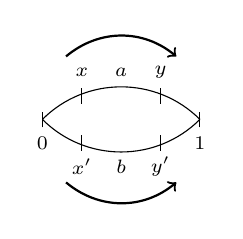
\begin{tikzpicture}
		\node (1) at (0,-0.3) {\scriptsize{$0$}};
		\node (2) at (2,-0.3) {\scriptsize{$1$}};
		\node (a) at (1,0.6) {\scriptsize{$a$}};
		\node (b) at (1,-0.6) {\scriptsize{$b$}};
		\node (x) at (0.5,0.6) {\scriptsize{$x$}};
		\node (y) at (1.5,0.6) {\scriptsize{$y$}};
		\node (x') at (0.5,-0.6) {\scriptsize{$x'$}};
		\node (y') at (1.5,-0.6) {\scriptsize{$y'$}};
		\draw (0,0) to [bend left = 45] (2,0);
		\draw (0,0) to [bend right = 45] (2,0);
		\draw (0.5,0.2) -- (0.5,0.4);
		\draw (1.5,0.2) -- (1.5,0.4);
		\draw (0.5,-0.2) -- (0.5,-0.4);
		\draw (1.5,-0.2) -- (1.5,-0.4);
		\draw (0,-0.1) -- (0,0.1);
		\draw (2,-0.1) -- (2,0.1);
		\draw[->,thick] (0.3,0.8) to [bend left = 40] (1.7,0.8);
		\draw[->,thick] (0.3,-0.8) to [bend right = 40] (1.7,-0.8);
\end{tikzpicture}
  		\end{center}
	\end{figure}
The description of $\fac{\trace{a+b}}$ is now as follow. Objects of $\fac{\trace{a+b}}$ are
traces, which can be either:
\begin{itemize}
	\item constant traces, $0$, $x$, $y$, $x'$, $y'$, $1$, for all points $x$, $y$, $x'$, $y'$ that we chose to distinguish in the picture of $a+b$.
	\item non constant and non maximal traces of the form $[0,x]$, $[x,y]$, $[y,1]$ etc.
	\item maximal traces $a$ and $b$.
\end{itemize}
We chose below to draw a picture of a subcategory of $\fac{\trace{a+b}}$, where $x$, $y$, $x'$ and $y'$ are any distinguished points of $a$ and $b$ as discussed before. The extension morphisms in $\fac{\trace{a+b}}$ are pictured below as arrows ; for instance, there is an extension morphism from the trace $[x,y]$ to $[0,y]$ and to $[x,1]$, among other extension morphisms: 
	\begin{figure}[H]
		\begin{center}
    				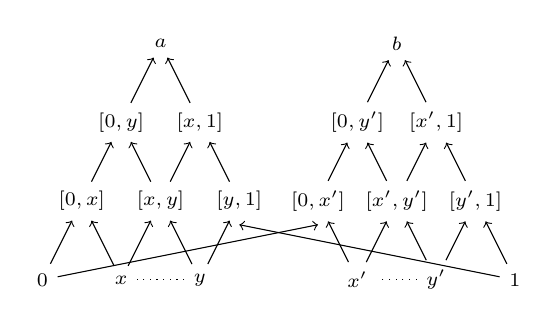
\begin{tikzpicture}[scale = 1]
		%\node at (3,-0.5) {\rotatebox{90}{\huge{\{}}};
		\node (0) at (0,0) {\scriptsize{$0$}};
		%\node (1) at (3,0) {$1$};
		\node (x) at (1,0) {\scriptsize{$x$}};
		\node (y) at (2,0) {\scriptsize{$y$}};
		\node (0x) at (0.5,1) {\scriptsize{$[0,x]$}};
		\node (y1) at (2.5,1) {\scriptsize{$[y,1]$}};
		\node (xy) at (1.5,1) {\scriptsize{$[x,y]$}};
		\node (0y) at (1,2) {\scriptsize{$[0,y]$}};
		\node (x1) at (2,2) {\scriptsize{$[x,1]$}};
		\node (a) at (1.5,3) {\scriptsize{$a$}};
		
		%\node (0) at (4,0) {$0$};
		\node (1) at (6,0) {\scriptsize{$1$}};
		\node (x') at (4,0) {\scriptsize{$x'$}};
		\node (y') at (5,0) {\scriptsize{$y'$}};
		\node (0x') at (3.5,1) {\scriptsize{$[0,x']$}};
		\node (y'1) at (5.5,1) {\scriptsize{$[y',1]$}};
		\node (x'y') at (4.5,1) {\scriptsize{$[x',y']$}};
		\node (0y') at (4,2) {\scriptsize{$[0,y']$}};
		\node (x'1) at (5,2) {\scriptsize{$[x',1]$}};
		\node (b) at (4.5,3) {\scriptsize{$b$}};
		
		%\draw[dotted] (0) -- (x);
		\draw[dotted] (y) -- (x);
		\draw[dotted] (y') -- (x');
		%\draw[dotted] (y) -- (1);
		
		\draw[->] (0) -> (0x);
		\draw[->] (x) -> (0x);
		\draw[->] (1) -> (2.5,0.7);
		\draw[->] (y) -> (y1);
		\draw[->] (x) -> (xy);
		\draw[->] (y) -> (xy);
		\draw[->] (0x) -> (0y);
		\draw[->] (xy) -> (0y);
		\draw[->] (y1) -> (x1);
		\draw[->] (xy) -> (x1);
		\draw[->] (0y) -> (a);
		\draw[->] (x1) -> (a);
		
		\draw[->] (0) -> (3.5,0.7);
		\draw[->] (x') -> (0x');
		\draw[->] (1) -> (y'1);
		\draw[->] (y') -> (y'1);
		\draw[->] (x') -> (x'y');
		\draw[->] (y') -> (x'y');
		\draw[->] (0x') -> (0y');
		\draw[->] (x'y') -> (0y');
		\draw[->] (y'1) -> (x'1);
		\draw[->] (x'y') -> (x'1);
		\draw[->] (0y') -> (b);
		\draw[->] (x'1) -> (b);
	\end{tikzpicture}
  		\end{center}
	\end{figure}
	
The only difference between $\fac{\trace{a+b}}$ and $\env{\trace{a+b}}$ is that $\env{\trace{a+b}}$ only has one top object, which corresponds to the pair $(0,1)$. That is, it is of the following form:
	\begin{figure}[H]
		\begin{center}
    			\input{images/DirHom/EnvExa}
  		\end{center}
	\end{figure}
	
Now, we can picture $\nathomolbw{1}{a+b}$, by applying the
homology functor on the trace spaces from the starting point to the end
point of the traces. For instance, the trace
space $\tracep{a+b}{x}{y}$ (respectively 
$\tracep{a+b}{0}{y}$) corresponding to the trace $[x,y]$ 
(respectively $[0,y]$) in the diagram
above, is just a point, hence has zeroth homology group equals to $\R$
(respectively $\R$). 
All other zeroth homology groups are also $\R$ with the exception of 
the ones corresponding to the two maximal traces 
$a$ and $b$, going from $0$ to $1$. In that case, 
$\tracep{a+b}{0}{1}$ is composed of two points, that we can identify with
$a$ and $b$ themselves, and has $\R^2$ (or $\R[a,b]$ with the identification we just
made) as
zeroth homology group. Now the extension morphism from $[0,y]$ to $a$ induces
a map in homology which maps the only generator of $H_0(\tracep{a+b}{0}{y})$
to generator $a$ in $\R[a,b]$ as indicated in the picture below:
	\begin{figure}[H]
		\begin{center}
    			\input{images/DirHom/NHomExa}
  		\end{center}
	\end{figure}
Similarly, the first bimodule of homology $\nathomolhm{1}{a+b}$ is of the following form:
	\begin{figure}[H]
		\begin{center}
    				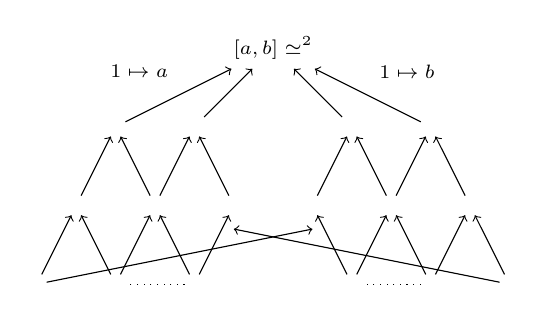
\begin{tikzpicture}[scale = 1]
		%\node at (3,-0.5) {};
		\node (0) at (0,0) {\scriptsize{$\R$}};
		%\node (1) at (3,0) {$1$};
		\node (x) at (1,0) {\scriptsize{$\R$}};
		\node (y) at (2,0) {\scriptsize{$\R$}};
		\node (0x) at (0.5,1) {\scriptsize{$\R$}};
		\node (y1) at (2.5,1) {\scriptsize{$\R$}};
		\node (xy) at (1.5,1) {\scriptsize{$\R$}};
		\node (0y) at (1,2) {\scriptsize{$\R$}};
		\node (x1) at (2,2) {\scriptsize{$\R$}};
		\node (a) at (3,3) {\scriptsize{$\R[a,b]\simeq\R^2$}};
		
		%\node (0) at (4,0) {$0$};
		\node (1) at (6,0) {\scriptsize{$\R$}};
		\node (x') at (4,0) {\scriptsize{$\R$}};
		\node (y') at (5,0) {\scriptsize{$\R$}};
		\node (0x') at (3.5,1) {\scriptsize{$\R$}};
		\node (y'1) at (5.5,1) {\scriptsize{$\R$}};
		\node (x'y') at (4.5,1) {\scriptsize{$\R$}};
		\node (0y') at (4,2) {\scriptsize{$\R$}};
		\node (x'1) at (5,2) {\scriptsize{$\R$}};
		%\node (b) at (4.5,3) {\scriptsize{$\R[a,b]\simeq\R^2$}};
		
		\node at (1.3,2.7) {\scriptsize{$1 \mapsto a$}};
		\node at (4.7,2.7) {\scriptsize{$1 \mapsto b$}};
		
		%\draw[dotted] (0) -- (x);
		\draw[dotted] (y) -- (x);
		\draw[dotted] (y') -- (x');
		%\draw[dotted] (y) -- (1);
		
		\draw[->] (0) -> (0x);
		\draw[->] (x) -> (0x);
		\draw[->] (1) -> (2.5,0.7);
		\draw[->] (y) -> (y1);
		\draw[->] (x) -> (xy);
		\draw[->] (y) -> (xy);
		\draw[->] (0x) -> (0y);
		\draw[->] (xy) -> (0y);
		\draw[->] (y1) -> (x1);
		\draw[->] (xy) -> (x1);
		\draw[->] (0y) -> (a);
		\draw[->] (x1) -> (a);
		
		\draw[->] (0) -> (3.5,0.7);
		\draw[->] (x') -> (0x');
		\draw[->] (1) -> (y'1);
		\draw[->] (y') -> (y'1);
		\draw[->] (x') -> (x'y');
		\draw[->] (y') -> (x'y');
		\draw[->] (0x') -> (0y');
		\draw[->] (x'y') -> (0y');
		\draw[->] (y'1) -> (x'1);
		\draw[->] (x'y') -> (x'1);
		\draw[->] (0y') -> (a);
		\draw[->] (x'1) -> (a);
	\end{tikzpicture}
  		\end{center}
	\end{figure}



\section{Homology of diagrams}
\label{sec:homdiag}

	\subsection{Category of diagrams and functoriality}
	
	The first requirement of a homology theory is that it should be functorial. Natural systems and bimodules are both particular case of diagrams with values in a specified category $\M$ (in our case, $\M$ is $\setcat$, $\group$, $\modu{\R}$, $\topo$ or $\topo_\ast$), i.e., a functor from any small category to $\M$. That will be the category where our directed homotopy and homology functor will live.
	
	We define $\diagr{\M}$ the category whose:
\begin{itemize}
	\item objects are \textbf{diagrams}, i.e., functors from any small category $\C$ to $\M$,
	\item morphisms from $\map{F}{\C}{\M}$ to $\map{G}{\D}{\M}$ are pairs $(\Phi,\sigma)$ where
		\begin{itemize}
			\item $\Phi$ is a functor from $\C$ to $\D$,
			\item $\sigma$ is a natural transformation from $F$ to $G\circ\Phi$.
		\end{itemize}
	\item the identity on $\map{F}{\C}{\M}$ is $id_F = (id_\C,1_F)$ where
		\begin{itemize}
			\item $id_C$ is the identity functor on $\C$,
			\item $1_F$ is the identity natural transformation on $F$.
		\end{itemize}
	\item the composition is defined as follow: $(\Psi,\tau)\circ(\Phi,\sigma)$, where $\map{(\Phi,\sigma)}{(\map{F}{\C}{\M})}{(\map{G}{\D}{\M})}$ and $\map{(\Psi,\tau)}{(\map{G}{\D}{\M})}{(\map{H}{\E}{\M})}$, is $(\Psi\circ\Phi, (\tau_{\Phi(c)}\circ\sigma_c)_{c\in\ob{\M}})$.
\end{itemize}

\begin{prop}
	$\overrightarrow{BT}$ (resp. $\overrightarrow{NT}$) extends to a functor from $\dtop$ to $\diagr{\topo}$ (resp. $\diagr{\topo_\ast}$).
\end{prop}

\begin{proof}
	Let us do it for $\overrightarrow{NT}$.
	If $\map{f}{X}{Y}$ is a dimap, we define $\map{\tracebw{f} =(\Phi,\sigma)}{\tracebw{X}}{\tracebw{Y}}$ as follow:
		\begin{itemize}
			\item $\map{\Phi}{\fac{\trace{X}}}{\fac{\trace{Y}}}$ such that $\Phi(\tra{\gamma}) = \tra{f\circ \gamma}$ and $\Phi(\tra{\alpha}, \tra{\beta}) = (\tra{f\circ\alpha}, \tra{f\circ\beta})$
			\item if $\gamma$ is a dipath from $x$ to $y$, $\map{\sigma_{\tra{\gamma}}}{\tracep{X}{x}{y}}{\tracep{Y}{f(x)}{f(y)}}$ ~~ $\tra{\rho} \mapsto \tra{f\circ\rho}$. $\sigma_{\tra{\gamma}}$ does not depend on $\gamma$ but only on its end points.
		\end{itemize}
		It is easy to check this defines a functor.
	\end{proof}
	
	\begin{coro}
	The following extend to functors:
	\begin{itemize}
		\item $\overrightarrow{\Pi}_1$ with values in $\diagr{\setcat}$,
		\item $\overrightarrow{\Pi}_2$ with values in $\diagr{\group}$,
		\item $\overrightarrow{\Pi}_n$ for $n \geq 2$ with values in $\diagr{\Ab}$,
		\item $\overrightarrow{NH}_n$ and $\overrightarrow{BH}_n$ for every $n$, with values in $\diagr{\modu{\R}}$.
	\end{itemize}
	\end{coro}

	
	\subsection{(Co)completeness and additivity axiom}
	
	Let us look at the limits and the colimits of $\diagr{\M}$. First, as it is well known \cite{maclane78}, $\cat$ is complete. If $\C$ is a small category and $\map{F}{\C}{\cat}$ a diagram in $\cat$, the limit of $F$ is the category $\Lim{F}$ whose:
\begin{itemize}
	\item objects are the families $(x_c)_{c\in\ob{\C}}$ where $x_c \in \ob{F(c)}$ and for every morphism $\map{f}{c}{c'}$ of $\C$, $F(f)(x_c) = x_{c'}$,
	\item morphisms from $(x_c)_{c\in\ob{\C}}$ to $(y_c)_{c\in\ob{\C}}$ are the families $(g_c)_{c\in\ob{\C}}$ where $\map{g_c}{x_c}{y_c}$ and for every morphism $\map{f}{c}{c'}$ of $\C$, $F(f)(g_c) = g_{c'}$,
	\item composition $(h_c)_{c\in\ob{\C}}\circ(g_c)_{c\in\ob{\C}}$ is $(h_c\circ g_c)_{c\in\ob{\C}}$,
	\item the identity of $(x_c)_{c\in\ob{\C}}$ is $(\id_{x_c})_{c\in\ob{\C}}$.
\end{itemize}
together with the projection functors.

A functor from $\C$ to $\M$ will be called a \textbf{$\C$-diagram of $\M$}. We say that a category \textbf{$\M$ has $\C$-limits} if every $\C$-diagram of $\M$ has a limit.

\begin{prop} Let $\C$ be a small category. If $\M$ has $\C$-limits then $\diagr{\M}$ has $\C$-limits.
\end{prop}


\begin{proof}~
Suppose that $\M$ has $\C$-limits. Let $\map{F}{\C}{\diagr{\M}}$. $F$ induces a $\C$-diagram in $\cat$ $\map{G_F}{\C}{\cat}$ as follow: 
		\begin{itemize}
			\item[$\bullet$] $G_F(c)$ is the domain of $F(c)$,
			\item[$\bullet$] $G_F(f)$ is the first component of $F(f)$.
		\end{itemize}
As $\cat$ is complete, $G_F$ has a limit $(\Lim{G_F},\map{\pi_c}{\Lim{G_F}}{G(c)})$. Now, the limit of $F$ is the functor $\map{\Lim{F}}{\Lim{G_F}}{\M}$ such that:
		\begin{itemize}
			\item[$\bullet$] $\Lim{F}((x_c)_{c\in\ob{\C}})$ is the limit of the functor which maps
				\begin{itemize}
					\item[$*$] every $c\in\ob{\C}$ to $F(c)(x_c)$,
					\item[$*$] every $\map{f}{c}{c'}$ of $\C$ to the component of $x_c$ in the second component of $F(f)$ (which is a natural transformation).
				\end{itemize}
Such a limit exists because $\M$ has $\C$-limits.
			\item[$\bullet$] $\Lim{F}((g_c)_{c\in\ob{\C}})$ (where $\map{g_c}{x_c}{y_c}$) 
is the unique morphism of $\M$ defined below. As $\Lim{F}((y_c)_{c\in\ob{\C}})$ is a limit in $\M$, it makes every such diagram:
			\begin{center}
	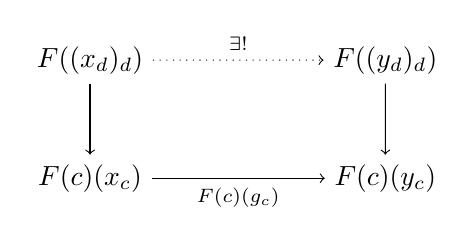
\begin{tikzpicture}[scale=1.5]
		\node (A) at (0,1) {$\Lim{F}((x_d)_d)$};
		\node (B) at (2.5,1) {$\Lim{F}((y_d)_d)$};
		\node (C) at (0,0) {$F(c)(x_c)$};
		\node (D) at (2.5,0) {$F(c)(y_c)$};
		\path[->,dotted,font=\scriptsize]
		(A) edge node[above]{$\exists ! $} (B);
		\path[->,font=\scriptsize]
		(A) edge node[left]{$$} (C)
		(B) edge node[right]{$$} (D)
		(C) edge node[below]{$F(c)(g_c)$} (D);
	\end{tikzpicture}
	\end{center}
commutative, together with the projection maps $$\map{(\pi_c,(\sigma_{c,(x_d)_{d}})_{(x_d)_d\in\ob{\Lim{G_F}}})}{\Lim{F}}{F(c)}$$ where $\map{\sigma_{c,(x_d)_{d}}}{\Lim{F}((x_d)_d)}{F(c)(x_c)}$ is the projection map coming from the fact that $\Lim{F}((x_d)_d)$ is a limit.
		\end{itemize}
\end{proof}

\begin{coro}
If $\M$ is complete then $\diagr{\M}$ is complete.
\end{coro}


We have a similar result for colimits.
\begin{prop}
If $\M$ is cocomplete then $\diagr{\M}$ is cocomplete.
\end{prop}

The colimits are very technical but follow the same ideas as for the limits: compute the colimit in $\cat$ and then construct a diagram on this colimit using colimits in $\M$. The main difference is that the latter colimits are not colimits of $\C$-diagrams much as in limits and are much more complicated. We will not prove this result, our only interest here are coproducts for the additivity axiom. Those are really simple:

\begin{prop}
$\diagr{\M}$ always has coproducts.
\end{prop}

Those coproducts are computed as follow. Given a family $(\map{F_i}{\C_i}{\M})_{i\in I}$ of diagrams, its coproduct is the diagram whose:
\begin{itemize}
	\item domain is the category which is the disjoint union of the $\C_i$,
	\item the value of the functor of the $i$th component of the disjoint union is the value of $F_i$.
\end{itemize}

Recall now that the coproduct in $\dtop$ is also the disjoint union. So if $X = \sqcup X_i$ is a disjoint union of d-spaces, then $\tracep{X}{a}{b}$ is:
\begin{itemize}
	\item $\varnothing$ if $a$ and $b$ are not in the same $X_i$,
	\item $\tracep{X_i}{a}{b}$ if $a, b \in X_i$.
\end{itemize}
Put another way, the trace category $\trace{X}$ is the disjoint union of the $\trace{X_i}$. Consequently:

\begin{prop}[\textbf{Additivity axiom}]
$\overrightarrow{NT}$, $\overrightarrow{BT}$, $\overrightarrow{NH}_n$ and $\overrightarrow{BH}_n$ preserve coproducts.
\end{prop}
	
	\subsection{Null objects and dimension axioms}
	
	One reason why homology works so well is that it is with values in Abelian categories. $\diagr{\M}$ is (essentially) never Abelian: for example, an Abelian category is required to have a zero object, that is, an object which is both initial and final (for example, any trivial group in $\Ab$). In $\diagr{\M}$, the initial object is always the empty diagram. When $\M$ has a initial object, the initial object of $\diagr{\M}$ is the diagram from $\textbf{1}$, the category with one object and one morphism, to $\M$, which maps the only object of $\textbf{1}$ to the initial object of $\M$. Consequently, in this case, the initial and the final objects cannot coincide and $\diagr{\M}$ is not Abelian.
	
	Nevertheless, when $\M$ is Abelian (for example, if $\M = \modu{\R}$), there are particular diagrams that looks like zero objects: the diagrams $\map{F}{\C}{\M}$ such that for every object $c$, $F(c)$ is a zero object of $\M$. We will see later that they play the same role as a zero object in this case. We will call them \textbf{null diagrams}. In particular, the initial and the final objects of $\diagr{\M}$ are null. Consquently:
	
	\begin{prop}[Dimension axiom]
	For every $n \neq 1$, $\nathomolbw{n}{\ast}$ and $\nathomolhm{n}{\ast}$ are final and so, null.
	\end{prop}
	
	
	
	\subsection{Semi-exact categories and exact sequences}
	
	Among Eilenberg-Steenrod axioms, the exactness axiom, or more precisely, the more general statement that claims that homology must transform short exact sequences of chain complexes into long exact sequences is a purely algebraic statement, no topology is involved. For singular homology, this works because homology is defined as the homology of a chain complex in modules and that the category $\modu{\R}$ is Abelian. Actually, it seems unavoidable to be in an Abelian category to even be able to talk about chain complexes, kernels, images, exact sequences, and so on. Since categories of diagrams are not Abelian in general, we should turn to non-Abelian theories. In the next few subsections, we will study the theory from \cite{grandis91,grandis91b} which turns out to be the framework that will allow us to look at the theory of exact sequences in diagrams.
	
	Let $\A$ be a category. An \textbf{ideal} of $\A$ is a class of morphisms closed under left and right compositions by any morphism of $\A$. Let $N$ be an ideal of $\A$. We call the morphisms in $N$, the \textbf{null morphisms}. A \textbf{null object} is an object of $\A$ whose identity is null. We say that $N$ is \textbf{closed} if every null morphism factorizes through a null object, i.e., for every $\map{f}{a}{b} \in N$, there exists a null object $c$ and two morphisms $\map{g}{a}{c}$ and $\map{h}{c}{b}$ such that $f = h \circ g$.
	
	The class of linear maps which maps every element to zero is an ideal of $\modu{\R}$. In this case, the null objects are precisely the trivial modules. More generally, the class of morphisms which factorizes through a zero object of an Abelian category $\A$ (those morphisms are called zero morphisms) is an ideal of $\A$. By definition, this ideal is closed. Given a category $\M$ and an ideal $N$ of $\M$, the class $L_N$ of morphisms of diagrams $\map{(\Phi,\sigma)}{\map{F}{\C}{\M}}{\map{G}{\D}{\M}}$ such that for every $c$ object of $\C$, $\sigma_c \in N$ is an ideal of $\diagr{\M}$. The null objects are precisely the diagrams $\map{F}{\C}{\M}$ such that for every object $c$, $F(c)$ is a null object. In the case of $\modu{\R}$ and the ideal of zero morphisms, those null objects are what we called null diagrams previously. Also in this case, $L_N$ is closed since every null morphism from $\map{F}{\C}{\modu{\R}}$ to $\map{G}{\D}{\modu{\R}}$ factorizes through the diagram $\map{0_\D}{\D}{\modu{\R}}$ which maps every object of $\D$ to the trivial module.
	
	The \textbf{kernel} (with respect to $N$) of a morphism $\map{f}{a}{b}$ of $\A$ is (when it exists) the unique (up to isomorphism) morphism $\map{\ke{f}}{\Ke{f}}{a}$ such that: 
\begin{itemize}
	\item $f \circ \ke{f} \in N$,
	\item for every $\map{g}{c}{a}$ such that $f \circ g \in N$, there exists a unique $\map{h}{c}{\Ke{f}}$ such that $g = \ker{f} \circ h$
\end{itemize}
We define dually, the \textbf{cokernel} $\map{\cok{f}}{b}{\Cok{f}}$.

	In the case of an Abelian category with its ideal of zero morphisms, kernels and cokernels exist and are given by the kernels and cokernels of the Abelian structure. They then are a special case of the following:
	
	\begin{defi}[\cite{grandis91}]
	A \textbf{semiexact category} is a pair $(\A, N)$ where $N$ is a closed ideal of the category $\A$ such that every morphism of $\A$ has a kernel and a cokernel with respect to $N$.
	\end{defi}
	
	\begin{lemme} If $(\M, N)$ is semi-exact then $L_N$ is a closed ideal of $\diagr{\M}$ and $\diagr{\M}$ has kernels with respect to $L_N$.
	\end{lemme}
	
	\begin{proof} ~
\begin{itemize}
	\item \textbf{$L_N$ is an ideal:} because $N$ is.
	\item \textbf{$L_N$ closed:} we know by $3.7$ of \cite{grandis91} that in $\M$, $\map{f}{a}{b}$ is null if and only if $f$ factorizes through $\map{\ke{\id_b}}{\Ke{\id_b}}{b}$ and we know that $\Ke{\id_b}$ is a null object. So if $\map{(\Phi,\sigma)}{(\map{F}{\C}{\M})}{(\map{G}{\D}{\M})}$ is null then it factorizes through $0_{G}$ where 
	$\map{0_{G}}{\D}{\M}$ with $0_{G}(d) = \Ke{\id_{G(d)}}$ and $\map{0_{G}(f)}{0_{G}(d)}{0_{G}(d')}$ the unique morphism which makes this square commutative:
	\begin{center}
	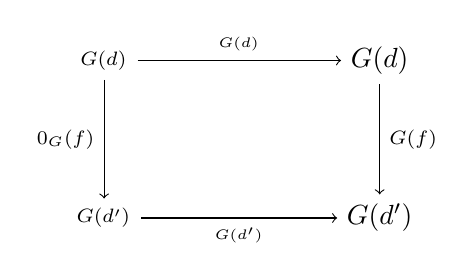
\begin{tikzpicture}[scale=1]
		\node (A) at (0,2) {$\Ke{\id_{G(d)}}$};
		\node (B) at (3.5,2) {$G(d)$};
		\node (C) at (0,0) {$\Ke{\id_{G(d')}}$};
		\node (D) at (3.5,0) {$G(d')$};
		\path[->,font=\scriptsize]
		(A) edge node[above]{$\ke{\id_{G(d)}}$} (B)
		(A) edge node[left]{$0_{G}(f)$} (C)
		(B) edge node[right]{$G(f)$} (D)
		(C) edge node[below]{$\ke{\id_{G(d')}}$} (D);
	\end{tikzpicture}
	\end{center}
	coming from the universal property of $\ker{\id_{G(d')}}$. You may note that this construction coincides with $0_\D$ defined in the case where $\M$ is Abelian.
	\item \textbf{kernels:} if $\map{(\Phi,\sigma)}{(\map{F}{\C}{\M})}{(\map{G}{\D}{\M})}$, we construct its kernel:
	$$\map{(\Phi_{\text{ker}},\sigma_{\text{ker}})}{(\map{F_{\text{ker}}}{\C_{\text{ker}}}{\M})}{(\map{F}{\C}{\M})}$$
	as follow.
		\begin{itemize}
			\item $\C_{\text{ker}} = \C$,
			\item $\Phi_{\text{ker}} = \id_{\C}$,
			\item $\map{F_{\text{ker}}}{\C}{\M}$ with $F_{\text{ker}}(c) = \Ke{\sigma_c}$ and $F_{\text{ker}}(f)$ the unique morphism which makes the left square 
			commutative:
			\begin{center}
			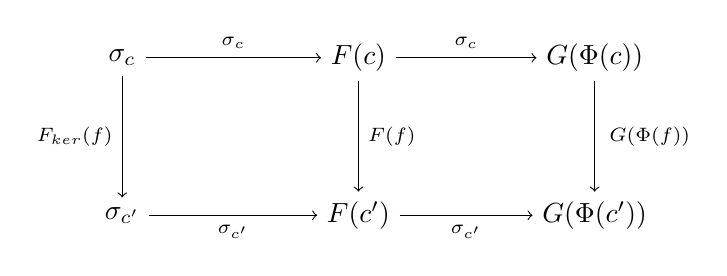
\begin{tikzpicture}[scale=1]
				\node (A) at (0,2) {$\Ke{\sigma_c}$};
				\node (B) at (3,2) {$F(c)$};
				\node (C) at (0,0) {$\Ke{\sigma_{c'}}$};
				\node (D) at (3,0) {$F(c')$};
				\node (E) at (6,0) {$G(\Phi(c'))$};
				\node (F) at (6,2) {$G(\Phi(c))$};
				\node (G) at (6.7,1) {\scriptsize{$G(\Phi(f))$}};
				\path[->,font=\scriptsize]
				(A) edge node[above]{$\ke{\sigma_c}$} (B)
				(A) edge node[left]{$F_{\text{ker}}(f)$} (C)
				(B) edge node[right]{$F(f)$} (D)
				(C) edge node[below]{$\ke{\sigma_{c'}}$} (D)
				(B) edge node[above]{$\sigma_c$} (F)
				(D) edge node[below]{$\sigma_{c'}$} (E)
				(F) edge (E);
			\end{tikzpicture}
			\end{center}
					coming from the universal property of $\ke{\sigma_{c'}}$,
			\item $(\sigma_{\text{ker}})_c = \ke{\sigma_c}$.
		\end{itemize}
\end{itemize}
\end{proof}

One may be wondering why nothing was said about the cokernels: the thing is that they are much more complicated. Remember that kernels in $\modu{\R}$ are actually equalizers and since the limits in $\diagr{\modu{\R}}$ are computed levelwise, it is natural that kernels are computed levelwise, i.e., the kernel in diagrams is a diagram of kernels. Dually, cokernels in $\modu{\R}$ are coequalizers, and remember that colimits are complicated in $\diagr{\M}$, so it is expected that cokernels in $\diagr{\M}$ are complicated too.

\begin{lemme} $\diagrmod{\R}$ has cokernels with respect to $L_N$. \end{lemme}

\begin{proof}
If $\map{(\Phi,\sigma)}{(\map{F}{\C}{\modu{\R}})}{(\map{G}{\D}{\modu{\R}})}$, we construct its cokernel:
	$$\map{(\Phi_{\text{cok}},\sigma_{\text{cok}})}{(\map{G}{\D}{\modu{\R}})}{(\map{G_{\text{cok}}}{\D_{\text{cok}}}{\modu{\R}})}$$
as follow:
		\begin{itemize}
			\item ${\D}_{\text{cok}} = {\D}$
			\item $\Phi_{\text{cok}} = \id_{\D}$
			\item Let $\Gamma = \{(R_d)_{d_\in \ob{\D}} \mid R_d$ submodule of  $G(d)$ containing all the elements of
$\Ima{\sigma_c}$ with $\Phi(c) = d$ and such that if $\map{f}{d}{d'}$ then $G(f)(R_{d}) \subseteq R_{d'}$\}. $\Gamma$ contains $(G(d))_{d\in\ob{\D}}$ and is closed under intersection. Define then $(H_d)_{d\in\ob{\D}}$ as the intersection of all the elements of $\Gamma$. Then $(H_d)_{d\in\ob{\D}}\in\Gamma$.

			We also define $\map{G_{\text{cok}}}{\D}{\modu{\R}}$ with $G_{\text{cok}}(d) = G(d)/H_d$ and $G_{\text{cok}}(f)([x]) = [G(f)(x)]$. This is well defined because $(H_d)_{d\in\ob{\D}}\in\Gamma$.
			\item $(\sigma_{\text{cok}})_d(x) = [x]$
		\end{itemize}
Actually, this construction is the coequalizer of $(\Phi,\sigma)$ and $(\Phi,(\map{0}{F(c)}{G(\Phi(c))})_{c\in\ob{\C}})$.
\end{proof}

\begin{prop} $(\diagrmod{\R},L_N)$ is semi-exact. \end{prop}


Being able to talk about null morphisms and (co)kernels, allows us to define exactness. The \textbf{image} of a morphism $f$ is given by $\ima{f} = \ke{\cok{f}}$ (or $\Ima{f} = \Ke{\cok{f}}$ for the corresponding object) and the \textbf{coimage} by $\coima{f} = \cok{\ke{f}}$ (or $\Coima{f} = \Cok{\ke{f}}$). The sequence 
\begin{center}
\begin{tikzpicture}
  \matrix (m) [matrix of math nodes,row sep=4em,column sep=4em,minimum width=2em]
  {
     
A &
B &
C
    \\};
  \path[-stealth]
    (m-1-1) edge node [above] {$f$} (m-1-2)
    (m-1-2) edge node [above] {$g$} (m-1-3);
\end{tikzpicture}
\end{center}
is said to be:
\begin{itemize}
	\item \textbf{of order two} if $g \circ f$ is a null morphism,
	\item \textbf{short exact} if $f = \ke{g}$ and $g = \cok{f}$
	\item \textbf{exact} if $\ima{f} = \ke{g}$.
\end{itemize}
\textbf{Chain complexe}s in a semi-exact category $\M$ are defined the same way as in abelian groups requiring that the sequence of morphisms $C_{n+1} \xrightarrow{~\partial_{n+1}~} C_{n} \xrightarrow{~~\partial_n~~} C_{n-1}$ be of order two for each $n$ \cite{grandis91b}. A morphism of chain complexes $\map{(f_n)_{n}}{(C_n,\partial_n)}{(C'_n,\partial'_n)}$ is given by morphisms $\map{f_n}{C_n}{C'_n}$ such that $\partial'_n\circ f_{n+1} = f_{n}\circ\partial_n$.  We denote this category by $C_\bullet(\M)$. This category is also semi-exact (the null morphisms being families of null morphisms in $\M$).

	
	\subsection{Homological categories and homology of diagrams}
	
	Now, to define homology of a chain complex in a certain category, we must be able to talk about sub-quotients as in the case of modules, i.e., if $K\subseteq H\subseteq G$ are modules, we can define $H/K$. This is not the case in general, for example in groups even if $H$ and $K$ are normal sub-groups of $G$, $H/K$ may not define a group... 
	
	A morphism which is the kernel (resp. the cokernel) of a morphism will be called a\textbf{normal mono} (resp. \textbf{normal epi}). In Abelian category, normal monos (resp. normal epis) are all the monos (resp. all the epis). In the case of modules, monos are injections and epis are surjections.
	
	\begin{prop} Normal monos in $(\diagr{\M},L_N)$ are the $(\Phi,\sigma)$ where $\Phi$ is an isofunctor (that is, a bijective-on-objects fully faithful functor, or an isomorphism in the category of small categories and functors) and every $\sigma_c$ is a normal mono in $(\M,N)$. Normal epis in $(\diagrmod{\R},L_N)$ are $(\Phi,\sigma)$ where $\Phi$ is an isofunctor and every $\sigma_c$ is surjective. \end{prop}
	
	\begin{proof}
	Consequence of the computation of kernels and cokernels.
	\end{proof}
	
	\begin{defi}[\cite{grandis91}]
We say that a morphism is \textbf{exact} if it factorizes as $n\circ q$ with $q$, a normal epi and $n$, a normal mono. Given two monos $m$ and $n$, we write $m \geq n$ if there is a morphism $k$ (that will be unique and monic) such that $n = m\circ k$.

A semi-exact category $({\A}, N)$ is said to be \textbf{homological} if:
\begin{itemize}
	\item normal monos and normal epis are closed under composition,
	\item if $\map{m}{b}{a}$ is a normal mono and $\map{q}{a}{c}$ is a normal epi such that $m \geq \ke{q}$ then $q \circ m$ is exact. 
	\end{itemize}
In this case, if $\map{m}{b}{a}$ and $\map{n}{c}{a}$ are two normal monos with $m \geq n$, and if we write $q$ for the unique normal epi (up to isomorphism) such that $n = \ke{q}$, the objects $\Coima{q\circ m}$ and $\Ima{q\circ m}$ are isomorphic. We call this object the \textbf{sub-quotient} of $a$ induced by $m\geq n$, and we denote it by $b/c$.
\end{defi}

In an Abelian category, by the epi-mono factorization, every morphism is exact. So, every Abelian category is homological. In the case of modules, normal monos are exactly sub-modules and $\geq$ is just the inclusion. So, the subquotient is really the quotient $b/c$ of submodules of $a$.

\begin{prop} $\diagrmod{\R}$ is homological.\end{prop}

\begin{proof}~
\begin{itemize}
	\item the normal monos (resp. epis) are closed under composition because those of $\modu{\R}$ are.
	\item let $\map{(\Phi,\sigma)}{(\map{F}{\C}{\modu{\R}})}{(\map{G}{\D}{\modu{\R}})}$ be a normal mono. Thus $\Phi$ is an isofunctor. As normal monos and normal epis are stable under composition with an isomorphism, we can suppose, without loss of generality, that $\Phi = id_{\C}$ and $\D = \C$. The same way we can take $\map{(\Psi,\tau)}{(\map{G}{\C}{\modu{\R}})}{(\map{H}{\E}{\modu{\R}})}$ a normal epi with $\Psi = id_{\C}$ and $\C = \E$ and so, $(\Psi,\tau)\circ(\Phi,\sigma) = (id_{\C},(\tau_c\circ\sigma_c)_{c\in\ob{\C}})$.
	
	In $\modu{\R}$, $\tau_c\circ\sigma_c = \iota_c\circ\eta_c$ where $\map{\eta_c = \tau_c\circ\sigma_c}{F(c)}{\Ima{\tau_c\circ\sigma_c}}$ which is surjective and $\map{\iota_c}{\Ima{\tau_c\circ\sigma_c}}{H(c)}$ the inclusion, which is injective. Since $(\eta_c)_{c\in\ob{\C}}$ and $(\iota_c)_{c\in\ob{\C}}$ are natural and so $(id_{\C},\eta)$ is a normal epi, $(id_{\C},\iota)$ is a normal mono and $(\Psi,\tau)\circ(\Phi,\sigma) = (id_{\C},\iota)\circ(id_{\C},\eta)$.
\end{itemize}
\end{proof}

Consequently, in $\diagrmod{\R}$, normal monos are (up to isomorphisms) diagrams of submodules, $\geq$ is just the inclusion of submodules levelwise, and subquotient is just levelwise subquotient.

With the subquotients, the kernels and the images, it is possible to define homology in a homological category:

\begin{defi}[\cite{grandis91b}]
For a chain complex $C = (C_n, \partial_n)$:
\begin{itemize}
	\item $Z_n(C) = \Ke{\partial_{n-1}}$
	\item $B_n(C) =  \Ima{\partial_n}$
	\item $H_n(C) = Z_n(C)/B_n(C)$
\end{itemize}
and those constructions are functorial.
\end{defi}

As we have seen, homology modules of a space are defined as the homology modules of the singular chain complex. We can do the same with our directed homology. Define $\map{\overrightarrow{BC}}{\dtop}{\diagr{C_{\bullet}(\modu{\R})}}$ composing $\overrightarrow{BT}$ with the functor $C$ which associate every space with its singular chain complex. Similarly, we can define $\map{\overrightarrow{NC}}{\dtop}{\diagr{C_{\bullet}(\modu{\R})}}$, using $\overrightarrow{NT}$ instead. Diagrams in chain complexes can be seen as chain complexes in diagrams, so we can assume that $\overrightarrow{BC}$ and $\overrightarrow{NC}$ take values in $C_{\bullet}(\diagrmod{\R})$. We can then apply $H_n$ functors:

\begin{prop}
For every $n \leq 0$, $H_n\circ\overrightarrow{BC} = \overrightarrow{BH}_{n+1}$ and $H_n\circ\overrightarrow{NC} = \overrightarrow{NH}_{n+1}$.
\end{prop}
	
	
	\subsection{About modularity and the exactness axiom}
	
	
	The result in Abelian category on transformations of short exact sequences in chain complexes into long sequences on homology can be extended in homological categories:

\begin{theo}[\cite{grandis91b}] 
\label{theo:sod}
Let $\M$ be a homological category. For every short exact sequence in $C_\bullet(\M)$:
\begin{center}
\begin{tikzpicture}
  \matrix (m) [matrix of math nodes,row sep=4em,column sep=4em,minimum width=2em]
  {
     
U &
V &
W
    \\};
  \path[-stealth]
    (m-1-1) edge node [above] {$m$} (m-1-2)
    (m-1-2) edge node [above] {$p$} (m-1-3);
\end{tikzpicture}
\end{center}
there exists a sequence of order two in $\M$: 
\begin{center}
\begin{tikzpicture}
  \matrix (m) [matrix of math nodes,row sep=4em,column sep=2.5em,minimum width=2em]
  {
     \cdots & 
H_{n}(V) &
H_{n}(W) &
H_{n-1}(U) &
H_{n-1}(V) &
\cdots
    \\};
  \path[-stealth]
    (m-1-1) edge node [above] {} (m-1-2)
    (m-1-2) edge node [above] {\scriptsize{$H_n(p)$}} (m-1-3)
    (m-1-3) edge node [above] {\scriptsize{$\partial_n$}} (m-1-4)
    (m-1-4) edge node [above] {\scriptsize{$H_{n-1}(m)$}} (m-1-5)
    (m-1-5) edge node [above] {} (m-1-6);
\end{tikzpicture}
\end{center}
which is natural in the short exact sequence.\\
Moreover, \cite{grandis91b} gives some conditions for this sequence to be exact. In particular, those conditions are always satisfied iff $\M$ is \textbf{modular}.
\end{theo}

Let us explain what modularity means in the case of diagrams. A \textbf{normal subobject} of $\map{F}{\C}{\modu{\R}}$ is a morphism of the form $(id_\C,\sigma)$ where every $\sigma_c$ is an inclusion into $F(c)$. The set of all normal subobjects of $F$ is a lattice whose order is inclusion, meet is intersection, join is union, $\bot$ is $\sigma_c = 0$ and $\top$ is $id_{F(c)}$. Moreover, it is a modular lattice, in the sense that if $X \leq B$ then $X \vee (A\wedge B) = (X\vee A)\wedge B$. We denote this lattice by $Nsb(F)$. If $\map{f}{F}{G}$ is a morphism in $\diagrmod{\R}$, we can define a Galois connection $(f_*,f^*)$ where:
\begin{itemize}
	\item $\map{f_*}{Nsb(F)}{Nsb(G)}$  with $f_*(m) = \Ima{f\circ m}$.
	\item $\map{f^*}{Nsb(G)}{Nsb(F)}$  with $f^*(n) = \Ke{((\cok n)\circ f)}$.
\end{itemize}
The condition of modularity can be expressed as every morphism $\map{f}{F}{G}$ satisfies:
\begin{itemize}
	\item[1)] for every $x \in Nsb(F)$, $f^*\circ f_*(x) = x \vee f^*(\bot)$.
	\item[2)] for every $y \in Nsb(G)$, $f_*\circ f^*(y) = y \wedge f_*(\top)$.
\end{itemize}
	
	\begin{prop}
In $\diagrmod{\R}$, $1)$ and $2)$ fail and so $\diagrmod{\M}$ is not modular, meaning there some long sequences in homology that are not exact.
\end{prop}

\begin{proof}~
\begin{itemize}
	\item[1)] Let:
		\begin{itemize}
			\item $F$ the functor from the discrete category $\textbf{2}$ with two objects to $\modu{\R}$ which sends every object to $\R$,
			\item $G$ the functor from the discrete category $\textbf{1}$ with one object to $\modu{\R}$ which sends this object to $\R$,
			\item $\map{f}{F}{G}$ the morphism $(\Phi,\sigma)$ where $\Phi$ sends every object of $\textbf{2}$ to the unique object of $\textbf{1}$ and $\sigma$ is the natural transformation from $F$ to $G\circ\Phi$ which is only composed of identities,
			\item $x$ the normal subobject of $F$ which is the functor from $\textbf{2}$ to $\modu{\R}$ which sends one object to $0$ and the other to $\R$.
		\end{itemize}
In this case, $$x \vee f^*(\bot) = x \neq F = f^*\circ f_*(x).$$
	\item[2)] Let:
		\begin{itemize}
			\item $F$ the functor from $\textbf{1}$ to $\modu{\R}$ which this object to $\R$,
			\item $G$ the functor from the category $\textbf{2'}$ with two objects $\{a,b\}$ and one non-identity morphism which goes from $a$ to $b$, to $\modu{\R}$ which sends each object to $\R$ and the morphism to identity,
			\item $\map{f}{F}{G}$ the morphism $(\Phi,\sigma)$ where $\Phi$ sends the unique object of $\textbf{1}$ to $a$ and $\sigma$ is the natural transformation from $F$ to $G\circ\Phi$ which is only composed of identities,
			\item $y$ the normal subobject of $G$ which is the functor from $\textbf{2'}$ to $\modu{\R}$ which sends $a$ to $0$, $b$ to $\R$ and the morphism to $0$.
		\end{itemize}
In this case, $$y \wedge f_*(\top) = y \neq 0_G = f_*\circ f^*(y).$$
where $\map{0_G}{\textbf{2'}}{\modu{\R}}$ which maps each object to $0$ and the morphism to $0$.
\end{itemize}
\end{proof}

	\subsection{About relative homology and short exact sequences}
	
	Finally, let us talk about relative homology now. We have seen that relative homology is defined as the homology of the quotient $C(X)/C(A)$, that is, as the cokernel of the inclusion $C(A) \hookrightarrow C(X)$. Since, in modules, normal monos are precisely injections, the sequence $C(A) \rightarrow C(X) \rightarrow C(X)/C(A)$ is short exact and so produces a long exact sequence in homology.
	In the case of d-spaces and diagrams, the inclusion $\map{\iota}{\chainhm{A}}{\chainhm{X}}$ is not a normal mono. So one can still look at the cokernel of $\iota$ and define $\chainhm{X}/\chainhm{A} = \Cok{\iota}$, but the sequence
	$$\chainhm{A} \xrightarrow{~\iota~} \chainhm{X} \xrightarrow{~\cok{\iota}~} \chainhm{X}/\chainhm{A}$$
	is not short exact. The reason is that the cokernel in diagrams is defined as a quotient, but we quotient possibly more than what is given by the injection of $\iota$. Intuitively, we expect that for object $(a,b)$ of $\env{\trace{X}}$, the value of the functor $\chainhm{X}/\chainhm{A}$ on $(a,b)$ to be somehow $C(\tracep{X}{a}{b})/C(\tracep{A}{a}{b})$. This is not the case and what we obtain is $C(\tracep{X}{a}{b})/M_{a,b}$ where $M_{a,b,n}$ is the free module generated by the triples $(\tra{\alpha},\sigma,\tra{\beta})$ where $\alpha$ is a dipath in $X$ from $a$ to $a'$, $\beta$ is a dipath in $X$ from $b'$ to $b$ and $\sigma \in C(\tracep{A}{a'}{b'})_n$. The idea is that we do not quotient by singular simplexes of traces inside $A$ but by singular simplexes of traces that goes through $A$ at some point. So, if we define $\chainhm{A \subseteq X}$ as $\Ke{\cok{\iota}}$, that is the chain complex in $\diagr{\modu{\R}}$ such that $\chainhm{A \subseteq X}_n$ from $\env{\trace{X}}$ to $\diagr{C_{\bullet}(\modu{\R})}$whose value on $(a,b)$ is $M_{a,b}$ defined above, then the following sequence:
	$$\chainhm{A \subseteq X} \xrightarrow{~\ke{\cok{\iota}}~} \chainhm{X} \xrightarrow{~\cok{\iota}~} \chainhm{X}/\chainhm{A}$$
	is short exact.
	
	
\section*{Conclusion and discussion}
	
	In this chapter, we have described two homology theories for d-spaces. They both follow the same idea: we look at trace spaces and how they evolve by extending traces. The only difference is the description of the evolution, which leads to either a natural system when evolution is describe by traces and the category of factorizations, or a bimodule when evolution is describe by pairs of points and the enveloping category. We thus have a homology theory with values in diagrams in modules. This category of diagrams is not abelian, and we thus cannot use the work on exact sequences directly. However, we have seen that this category is homological in Grandis' sense, and so we can develop a non-abelian theory of exact sequences, although not as nice as in the abelian case.
	
	
	A natural question now is what about the homotopy axiom. The first kind we could think about follows this idea: in classical algebraic topology, we have seen that a homotopy equivalence induces isomorphisms in homology. Actually, this result can be strengthened \cite{hatcher02}: a weak homotopy equivalence (continuous function that induces isomorphisms in homotopy groups) induces isomorphisms in homology. A direct extension of this result in our case would be: if for a dimap $\map{f}{X}{Y}$, $\map{\nathomot{n}{f}}{\nathomot{n}{X}}{\nathomot{n}{Y}}$ is an isomorphism for every $n$, then $\map{\nathomolbw{n}{f}}{\nathomolbw{n}{X}}{\nathomolbw{n}{Y}}$ is an isomorphism for every $n$. The problem with this statement is that the hypothesis is very strong. Since the category $\trace{X}$ keeps lots of information about $X$, an $f$ such that $\nathomot{n}{f}$ is an isomorphism is not that far from dihomeomorphism. The thing is that we did not explain yet how we will compare diagrams. What we just said means that isomorphism in $\diagr{\M}$ is not a nice way to compare diagrams of homology. Remember that we are interested in how the trace spaces evolve with time, and so we must design an equivalence that compares those diagrams following this idea.










